\documentclass{article}
\usepackage{graphicx}

\title{An Introduction to Elliptic Curves}
\author{William Gvozdjak}

\begin{document}

\maketitle
Elliptic curves are one of the excitements of the research math world right now. For example, Fermat’s Last Theorem, a notorious and extremely difficult result in number theory, was finally proven after over three centuries using elliptic curves. What really are elliptic curves, and why are they useful?
\begin{center}
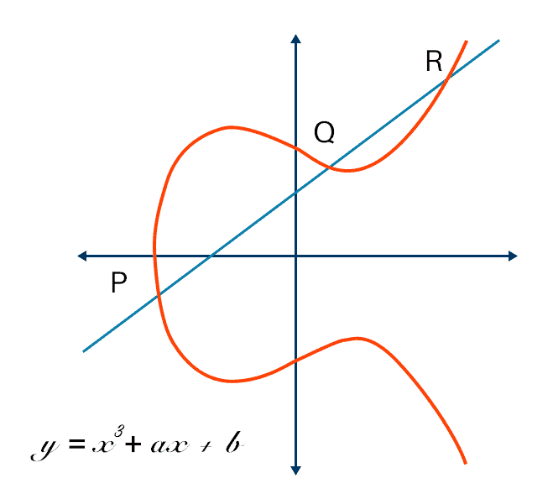
\includegraphics[scale=0.8]{images/curve3.png}
\end{center}
We first present an introductory question: is there a quick way to generate all primitive Pythagorean triples? In other words, is there an efficient method to generate all triples of positive integers $(a, b, c)$ where $c^2=a^2+b^2$, and $\gcd(a, b, c)=1$? How many solutions are there?

To answer this question, note that we can divide the above equation by $c^2$, giving us $1=\left(\frac{a}{c}\right)^2+\left(\frac{b}{c}\right)^2$. This is significant because this equation is now in the form of the equation of the unit circle! Therefore, we have shown that there is a one-to-one correspondence between primitive Pythagorean triples and ``rational points’’ with positive coordinates on the unit circle in the coordinate plane: points on the unit circle where both coordinates are positive, rational numbers.


How can we use this to general all primitive Pythagorean triples? We use a \textbf{projector}: we take an existing rational point, draw a line through that point, and use the second intersection of that line and the circle (``project’’ that point to another point on the circle). Our initial point will be a simple solution, such as $(-1, 0)$:

\begin{center}
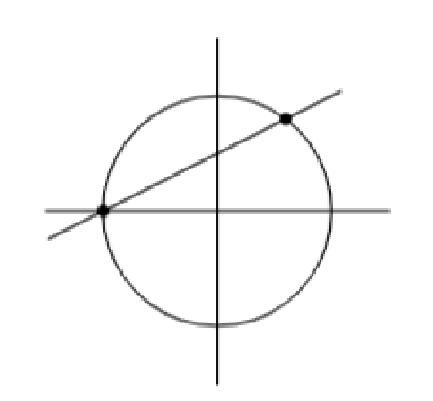
\includegraphics[scale=1]{images/curve1.png}
\end{center}

This new point must also be a rational point! This is not hard to show – we can solve the equation of the circle with the line, giving us a quadratic equation with rational coefficients. By Vieta’s formulas, as one solution is rational, the other solution must also be rational. Also, note that simply by varying the slope of the line that we project through to all rational numbers, we can actually generate \textit{all} rational solutions to $1=x^2+y^2$: if there is a rational point on $x^2+y^2=1$, then we can simply take the line through it and the point $(-1, 0)$ (this line is guaranteed to have rational slope).

Therefore, we have found a systematic way to find all primitive Pythagorean triples: take all lines with rational slope through the point $(-1, 0)$ and intersect them with the circle $x^2+y^2=1$, with the solutions with positive $x$ and $y$ coordinates resulting in primitive Pythagorean triples. Notice that this also proves that there are an infinite number of primitive Pythagorean triples, as there are an infinite number of rational numbers that we can choose as the slope.

Now, we look at a more complex problem. What is the set of all primitive triangles that have integer side lengths, integer area, and two sides with lengths that are in the ratio $3$ to $4$? Using Heron’s formula and some transformations, it is possible to prove that all such solutions are classified by the equation
\[y^2=x(x-9)(x-16).\]


An equation of this form is known as an \textbf{elliptic curve}: an equation of the form $y^2=p(x)$, where $p(x)$ is a polynomial of degree $3$ with $3$ distinct roots. As we wish to again generate all rational solutions to this equation, we will turn to the strategy that we used earlier for the primitive Pythagorean triples: the ``projections,’’ by looking for some sort of operation that will allow us to generate another solution.

\begin{center}
    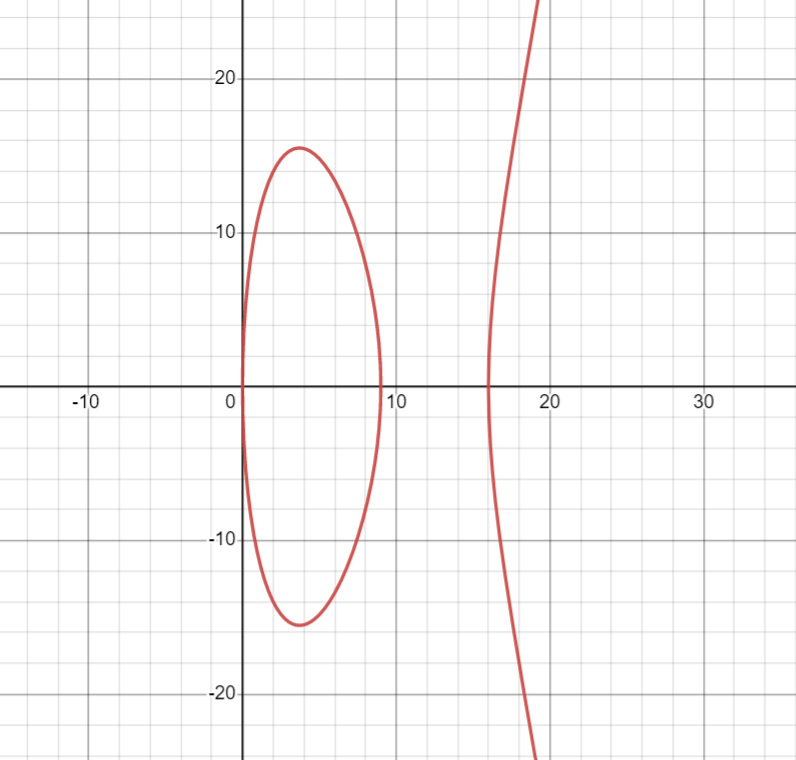
\includegraphics[scale=0.4]{images/ellipticCurves.png}
\end{center}

Inspired by our strategy with primitive Pythagorean triples, we may try to take a line and intersect it with the elliptic curve. Notice that if we do this, we end up with a cubic equation. However, unlike with the quadratic, this line not only needs to go through \textit{one} rational point, but \textit{two}: even if there is one rational solution, Vieta’s formulas does not guarantee that the last two solutions are necessarily rational. Therefore, we will define a new operation $\star$, which takes in two points $P$ and $Q$, and returns the third intersection point between the line $PQ$ and the elliptic curve. This requires some ``hacking’’ to rigorously define (e.g. what if $P=Q$, or $P$ and $Q$ have the same $x$-coordinate? Answering this requires the introduction of new ideas like a ``point at infinity’’), but this seems to satisfy most properties that we need.

\begin{center}
    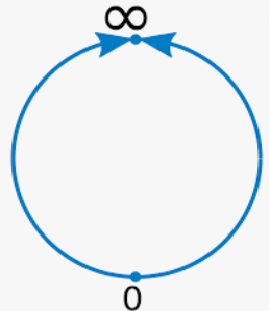
\includegraphics[scale=1.0]{images/curve4.png}
\end{center}

In reality, this operation behaves even nicer if we instead use the second intersection between the elliptic curve and the vertical line through $P\star Q$ (e.g. it behaves nicer with the point at infinity). Therefore, we have defined \textbf{elliptic curve addition}: the intersection of the elliptic curve with the vertical line through $P\star Q$. We have once again found a simple way to continuously generate solutions to our geometric problem with triangles!

This raises new questions: how long does the process of elliptic curve addition continue, until we start cycling back to points that we found before? Will it ever finish? Such ideas concern the \textbf{order} of elliptic curves. I highly encourage you to continue looking into such ideas and keep asking questions, as it appears that elliptic curves are the next big mathematical idea.
\end{document}